\chapter{Face data}

As a third and more sophisticated example, consider the data from a repetition priming experiment performed using event-related fMRI. Briefly, this is a 2x2 factorial study with factors `fame' and `repetition' where famous and non-famous faces were presented twice against a checkerboard baseline. The subject was asked to make fame judgements by making key presses. There are thus four event-types of interest; first and second presentations of famous and non-famous faces, which 
we denote N1, N2, F1 and F2. The experimental stimuli and timings of events are shown in Figures~\ref{face_stim} and \ref{face_timing}.
\begin{figure}
\begin{center}
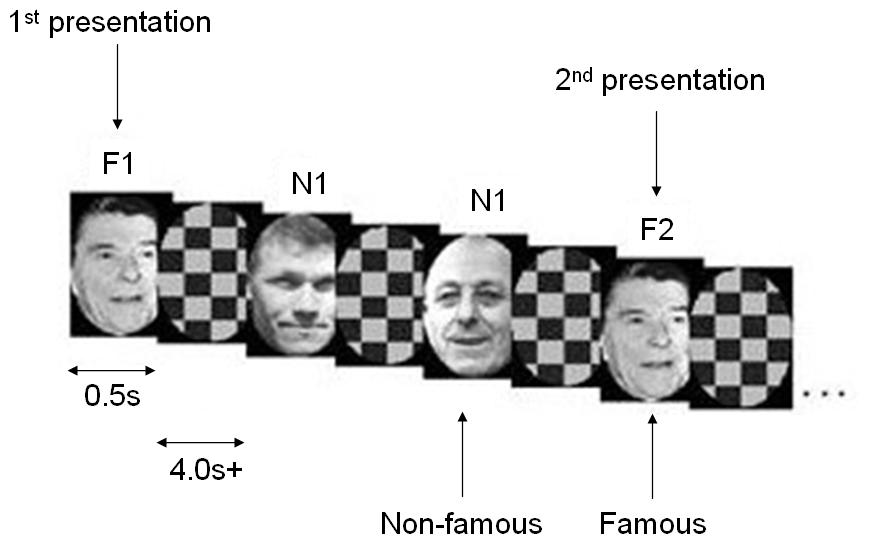
\includegraphics[width=120mm]{faces/face_stim}
\caption{\em Face repetition paradigm.  There were 2 presentations of 26 Famous and 26 Nonfamous Greyscale photographs, for 0.5s each, randomly intermixed. The 
minimal Stimulus Onset Asynchrony (SOA)=4.5s, with probability 2/3 (ie 1/3 null events). The subject made one of two 
right finger key presses denoting whether or not the subject thought the face was famous. \label{face_stim}}
\end{center}
\end{figure}
\begin{figure}
\begin{center}
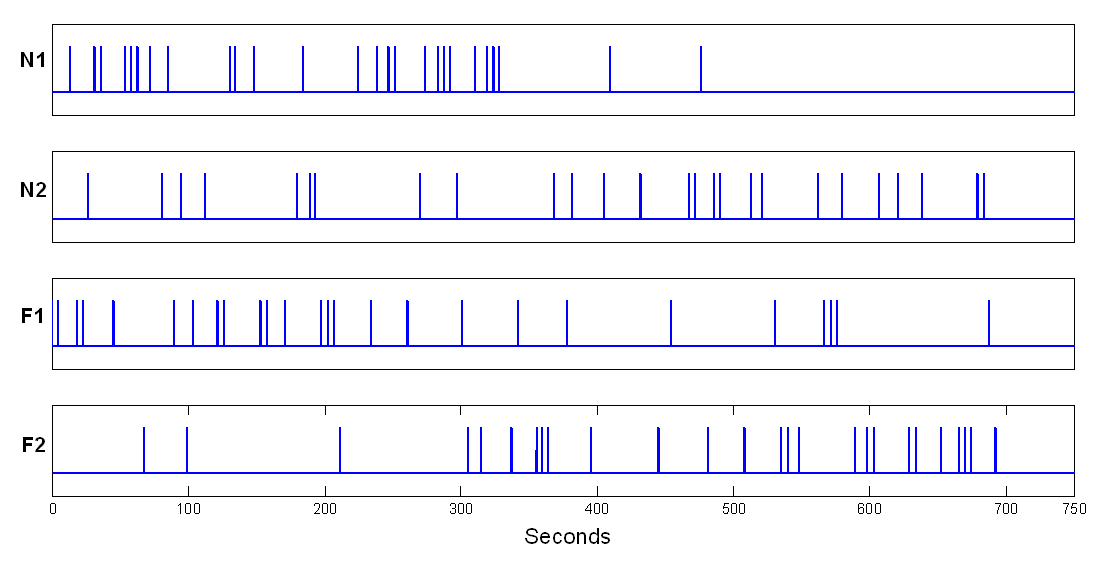
\includegraphics[width=120mm]{faces/face_timing}
\caption{\em Time series of events. \label{face_timing}}
\end{center}
\end{figure}

Images were acquired using continuous Echo-Planar 
Imaging (EPI) with TE=40ms, TR=2s and 24 descending slices (64x64 3x3$mm^2$), 3mm thick with a 1.5mm gap.
The data archive is available from 
This contains 351 Analyse format functional images
\verb!sM03953_0005_*.img! of dimension 
64x64x24 with 3mmx3mmx4.5mm voxels. A strucural 
image is also provided \verb!sM03953_0007.img! also in Analyse format.

To analyse the data, first create a new directory DIR 
\newline \verb!eg. c:\home\wpenny\fmri_analysis\face-rep\all!, in which to place the results
of your analysis. Then create 4 subdirectories (i) \verb!jobs!, 
(ii)  \verb!categorical!, (iii)  \verb!parametric! and (iv) \verb!bayesian!. As the analysis 
proceeds these directories will be filled with job-specification files, design matrices 
and models estimated using classical or Bayesian 
methods. 

As well as the classical/Bayesian 
distinction we will show how this 
data can be analysed from a parametric as well as a categorical perspective. We will look at the 
main effects of fame and repetition and in the 
parameteric analysis we will look at 
responses as a function of `lag', that is, the number of faces intervening between repetition of a specific face.

Start up matlab, enter your jobs directory and type {\em spm fmri} at the matlab prompt. SPM will then open in fMRI mode with three windows (1) the top-left or `command' window, (2) the 
bottom-left or `interactive' window
and (3) the right-hand or `graphics' window. 
Analysis 
then takes place in three major stages (i) 
spatial pre-processing, (ii) model specification, review 
and estimation and (iii) inference. These stages organise the buttons 
in SPM's base window.
\begin{figure}
\begin{center}
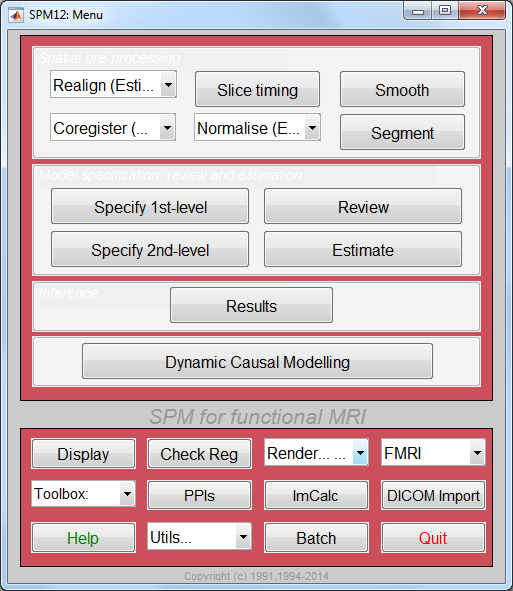
\includegraphics[width=100mm]{faces/command}
\caption{\em The SPM base window comprises 
three sections i) 
spatial pre-processing, (ii) model specification, review 
and estimation and (iii) inference. \label{command}}
\end{center}
\end{figure}

\section{Spatial pre-processing}

\subsection{Display}

Display eg. the first functional image using the 
`Display' button. Note orbitofrontal 
  and inferior temporal drop-out and ghosting. This 
  can be seen more clearly by selecting `brighten if necessary' from the `Effects' tab at the top of the 
  graphics window.
  \begin{figure}
\begin{center}
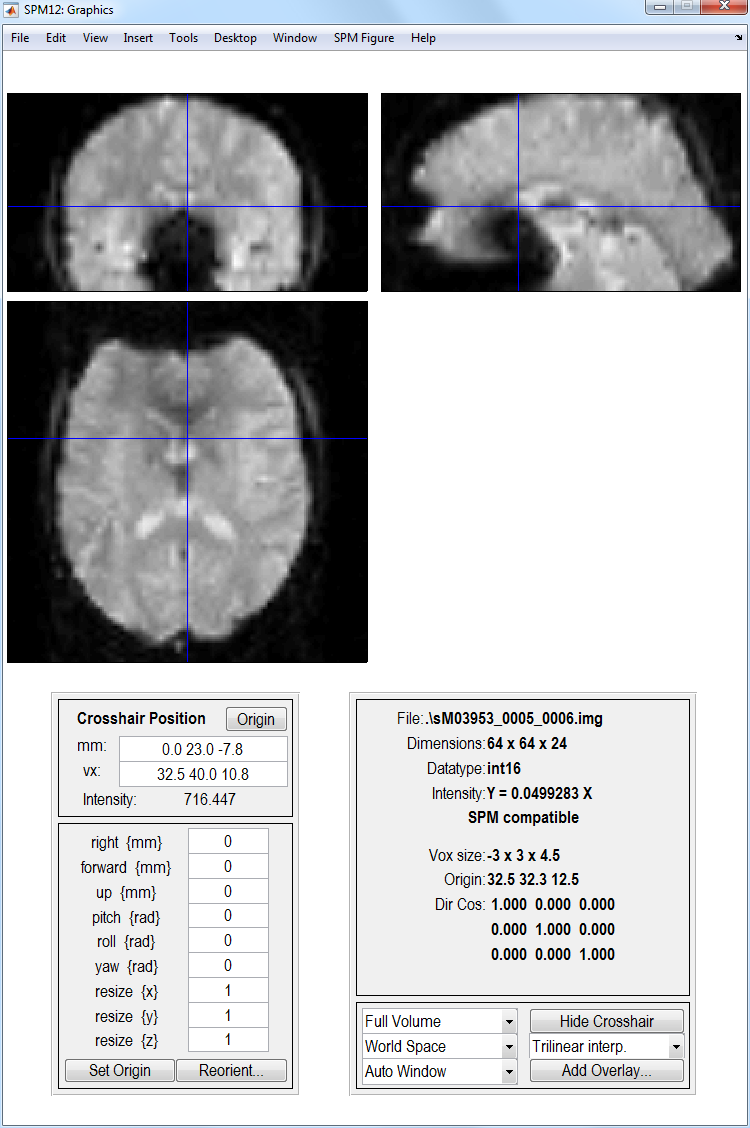
\includegraphics[width=100mm]{faces/dropout}
\caption{\em Signal dropout in EPI images. \label{dropout}}
\end{center}
\end{figure}

\subsection{Realignment}

Under the spatial pre-processing section of the SPM base window select `Realign' from the `Realign' pulldown menu. This will call up a realignment job specification 
in the graphics window.
Then
\bi
\item{Select `New Realign:Estimate and Reslice'}
\item{Open the newly created `Realign:Estimate and Reslice' option.}
\item{Highlight data, select `New Session', then highlight the newly created `Session' option.} 
\item{Select `Specify Files' and use the SPM file selector
to choose all of your functional images eg. \verb!sM03953_0005_*.img!.}
\item{Save the job file as eg. {\sf DIR/jobs/realign.mat}}.
\item{Press the RUN button in the graphics window.}
\ei
This 
will run the realign job which will write realigned images into the directory where the functional images
are. These new images will be prefixed with the letter `r'. SPM will then plot the estimated time series of translations and rotations shown in Figure~\ref{face_realign}. These data, the realignment parameters, are also saved to 
a file eg. \verb!rp_sM03953_0005_0006.txt!, so that these variables can be used as regressors when fitting GLMs. To prepare for this copy the file into the 
\verb!DIR\jobs\! directory and rename it \verb!movepars.txt!.
This allows movements effects to be discounted when
looking for brain activations.

SPM will also create a mean image eg. 
\verb!meansM03953_0005_0006.img! which will be used in the next
step of spatial processing - coregistration.
\begin{figure}
\begin{center}
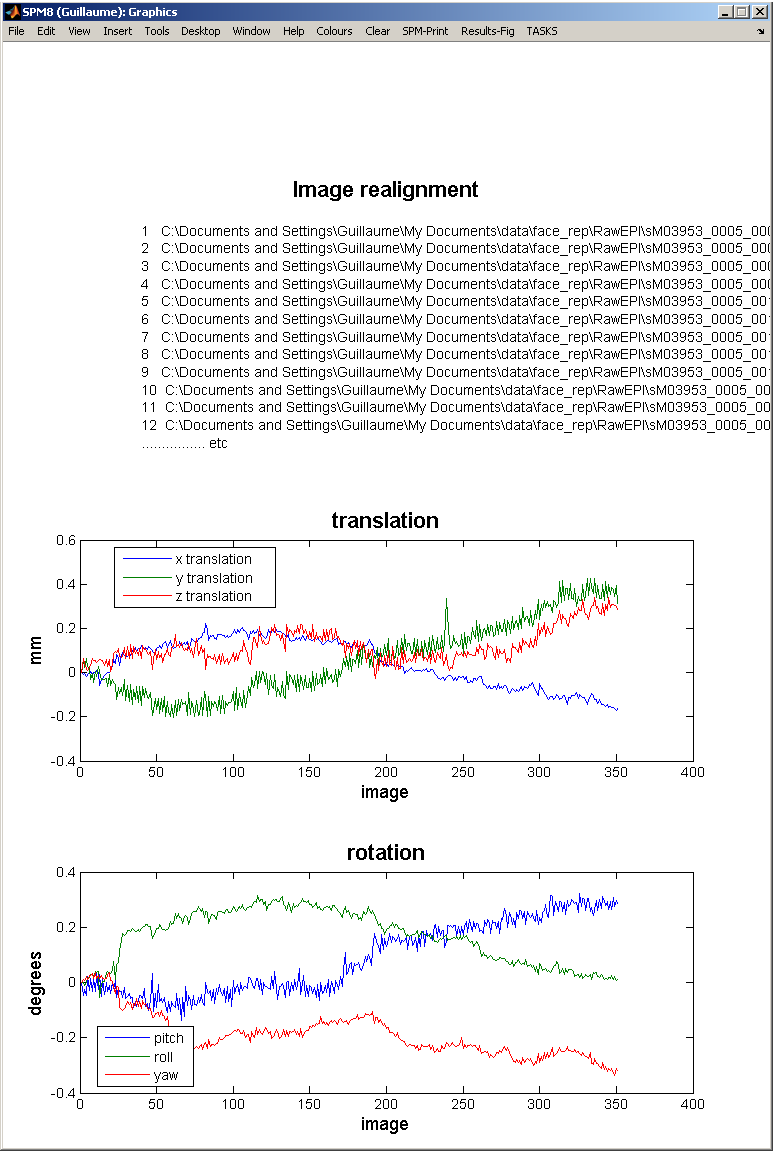
\includegraphics[width=100mm]{faces/realign}
\caption{\em Realignment of face data. Movement less than the size of a voxel, which for this data set is 3mm, is not considered problematic. \label{face_realign}}
\end{center}
\end{figure}

\subsection{Slice timing correction}

Press the `Slice timing' button. This will call up the specification of a slice timing job in the graphics 
window. 
\bi
\item{Open the `Slice Timing' option}
\item{Highlight `Data' and select `New Sessions'}
\item{Highlight the newly create `Sessions' option, `Specify Files' and select the
351 realigned functional images using the 
filter \verb!^r.*!.}
\item{Select `Number of Slices' and enter 24}
\item{Select TR and enter 2}
\item{Select TA and enter 2}
\item{Select `Slice order' and enter 24:-1:1}
\item{Select `Reference Slice', and enter 12}
\item{Save the job as \verb!slice_timing.mat! and press `Run'}
\ei
SPM will write slice-time corrected files with 
the prefix `a' in the functional data directory.

\subsection{Coregistration}

Press the `Coreg' button. This will call up the specification of a coregistration job in the graphics 
window. 

\bi
\item{Select New "Coreg:Estimate"}
\item{Double-click on the newly created Coreg:Estimate}
\item{Highlight `Reference Image' and then select the
 mean functional image
\verb!meansM03953_0005_0006.img!}
\item{Highlight `Source Image' and then select 
the structural image eg. \verb!sM03953_0007.img!.}
\item{Press the Save button and save the job as 
{\sf coreg.job}}
\item{Then press RUN}
\ei
SPM will then implement a coregistration between the structural and functional data that maximises the mutual information. The image in figure~\ref{aud_coreg} should then appear 
in the graphics window. SPM will have changed the header 
of the source file which in this case is the 
structural image \verb!sM03953_0007.img!.
\begin{figure}
\begin{center}
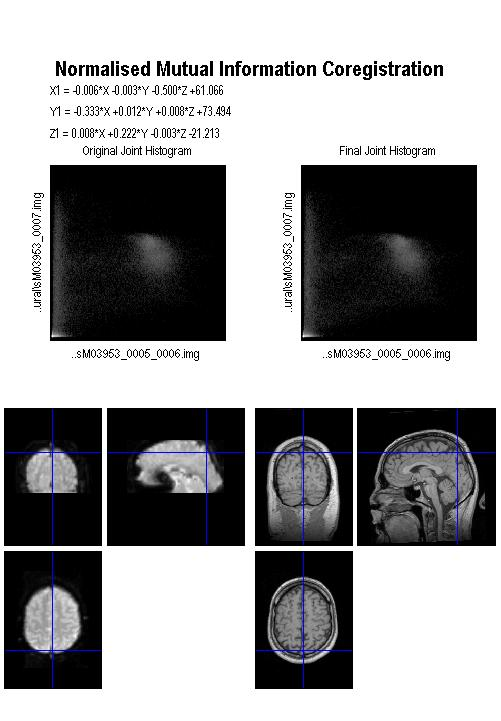
\includegraphics[width=100mm]{faces/coreg}
\caption{\em Mutual Information Coeregistration  of Auditory data. \label{aud_coreg}}
\end{center}
\end{figure}

\subsection{Segmentation}

Press the `Segment' button. This will call up the specification of a segmentation job in the graphics 
window. Highlight the Data field and then select 
the subjects coregistered anatomical image 
eg. \verb!sM03953_0007.img!. Save the job file
as {\sf segment.mat} and then press RUN.
SPM will segment the structural image using 
the default tissue probability maps as 
priors. 
SPM will create, by default, gray and white matter
images and bias-field corrected structral image.
These can be viewed using the CheckReg facility 
as described in the previous section (press segement 
and select . Figure \ref{face_gray} shows the gray matter image, \verb!c1sM03953_0007.img! along with the original structural.
\begin{figure}
\begin{center}
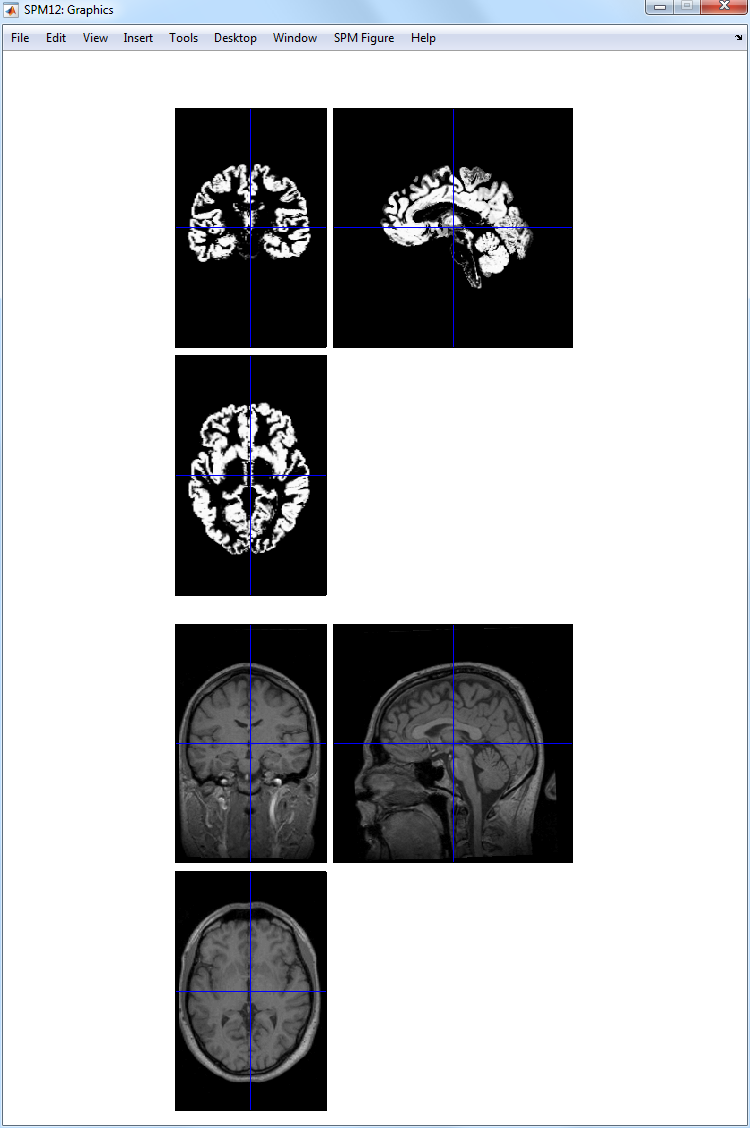
\includegraphics[width=100mm]{faces/gray}
\caption{\em Gray matter (top) produced by segmentation of structural image (below). \label{face_gray}}
\end{center}
\end{figure}

SPM will also write a spatial normalisation eg. 
\verb!sM03952_0007_seg_sn.mat! file in the 
original structural directory. This will be used 
in the next section to normalise the functional data. 


\subsection{Normalize}

Press the `Normalize' button. This will call up the specification of a normalise job in the graphics 
window. 

\bi
\item{Select a New "Normalise:Write" field. This 
allows previously estimated warps to be applied to 
a series of images.}
\item{Highlight `Data', select New "Subject"}
\item{Open `Subject', highlight `Parameter File' and 
select the \verb!sM03952_0007_seg_sn.mat! file that you 
created in the previous section}
\item{Highlight images to write and select all of the 
slice-time corrected, realigned functional images `arsM*.img'. Note: This can be done efficiently by changing the filter in the SPM file selector to \verb!^ar.*!. SPM will then only list those files beginning with the letter $r$ ie. those that have been realigned. You can then right click over the listed files, choose `Select all' and press `Done'.}
\item{Open `Writing Options', and change `Voxel sizes' from [2,2,2] to [3,3,3].\footnote{This step is not 
strictly necessary. It will write images out at 
a resolution closer to that at which they were acquired. 
This will speed up subsequent analysis and is necessary, for example, to make Bayesian fMRI analysis computationally efficient.}}
\item{Press `Save', save the job as normalise.mat and then
press `Run'.}
\ei
SPM will then write spatially normalised files to the 
functional data directory. These files have the prefix `w'.

If you wish to superimpose a subject's functional activations on their own anatomy\footnote{Beginners may wish to skip this step, and instead just superimpose functional activations on an `average structural image'.} you will also need to 
apply the spatial normalisation parameters to their 
(bias-corrected) anatomical image. To do this
\bi
\item{Press `Normalise', select New "Normalise:Write"}
\item{Open `Normalise: Write', highlight `Data', select 
New "Subject"}
\item{Open `Subject'}
\item{Highlight `Parameter File', select the  \verb!sM03952_0007_seg_sn.mat! file that you 
created in the previous section, press `Done'.}
\item{Highlight `Images to Write', select the 
bias-corrected structural eg. \verb!msM03952_0007.img!, press `Done'.}
\item{Open `Writing Options', select voxel sizes and 
change the default [2 2 2] to [1 1 1] which better matches the original resolution of the images [1 1 1.5].}
\item{Save the job as \verb!norm_struct.mat! and press `Run'}.
\ei

\subsection{Smoothing}

Press the `Smooth' button\footnote{The smoothing step is unnecessary if you are only interested in Bayesian analysis of your functional data.}. This will call up the specification of a smooth job in the graphics 
window.

\bi
\item{Open `Smooth', select `Images to Smooth' and then 
select the spatially normalised files created in the 
last section eg. {\sf war*.img}. }
\item{Save the job as {\sf smooth.mat} and press `Run'.}
\ei
This will smooth the data by 8mm in each direction, 
the default smoothing kernel width.
\begin{figure}
\begin{center}
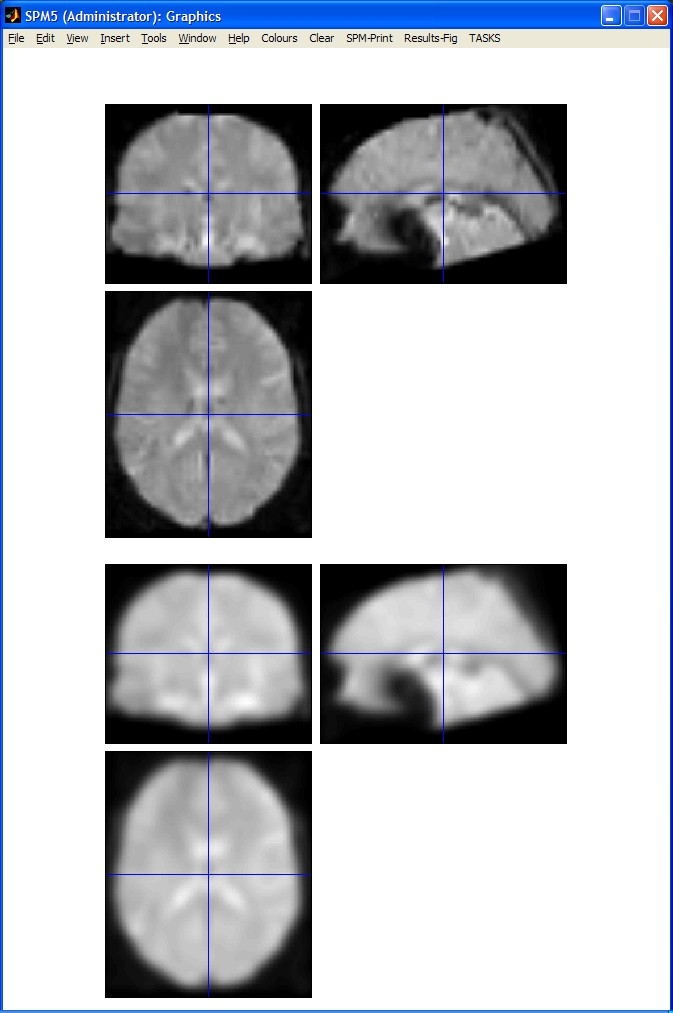
\includegraphics[width=100mm]{faces/smooth}
\caption{\em Functional image (top) and 8mm-smoothed functional image (bottom). These images were plotted using SPM's `CheckReg' facility. \label{face_smooth}}
\end{center}
\end{figure}

\section{Modelling categorical responses}


Before setting up the design matrix we must first 
load the Stimulus Onsets Times (SOTs) and movement
parameters into matlab. SOTs are stored in the 
\verb!sots.mat! file in a 
cell array such that eg. \verb!sot{1}! contains 
stimulus onset times in TRs for event type 1, which is N1. Event-types 2,3 and 4 are N2, F1 and F2\footnote{Also included included with this data set are variables describing two event-types of no interest - the (rare) errors made by this subject on the fame-judgement task. 
We will not, however, be using these in our analyses.}.

\bi
\item{At the matlab command prompt type `load sots'}
\item{Then type `load movepars.txt'}
\ei

Now press the `Specify 1st-level' button. This will call up the specification of a fMRI specification job in the graphics window. Then
\bi
\item{Open the fMRI model specification option}
\item{Open the `Timing paramaters' option}
\item{Highlight `Units for design' and select `Scans'}
\item{Highlight `Interscan interval' and enter 2}
\item{Highlight `Microtime resolution' and enter 24}
\item{Highlight `Microtime onset' and enter 12. These last two options make the creating of regressors commensurate with the slice-time correction we have 
applied to the data.}
\item{Highlight `Data and Design' and select `New Subject/Session'. Then open the newly created `Subject/Session' option.}
\item{Highlight `Scans' and use SPM's file selector to 
choose the 351 smoothed, normalised, slice-time corrected, realigned functional images ie  \verb!swarsM.img!. These can be selected 
easily using the \verb!^swar.*'! filter, and select all. Then press `Done'.}
\item{Highlight `Conditions' and select `New condition'\footnote{It is also possible to enter information about all of the conditions in one go. This requires much less button pressing and can be implemented by highlighting the `Multiple conditions' option and then
selecting the {\sf all-conditions.mat} file.}}
\item{Open the newly created `Condition' option. Highlight `Name' and enter `N1'. Highlight `Onsets' and enter `sot\{1\}'. Highlight `Durations' and enter 0.}
\item{Highlight `Conditions' and select `New condition'}
\item{Open the newly created `Condition' option. Highlight `Name' and enter `N2'. Highlight `Onsets' and enter `sot\{2\}'. Highlight `Durations' and enter 0.}
\item{Highlight `Conditions' and select `New condition'}
\item{Open the newly created `Condition' option. Highlight `Name' and enter `F1'. Highlight `Onsets' and enter `sot\{3\}'. Highlight `Durations' and enter 0.}
\item{Highlight `Conditions' and select `New condition'}
\item{Open the newly created `Condition' option. Highlight `Name' and enter `F2'. Highlight `Onsets' and enter `sot\{4\}'. Highlight `Durations' and enter 0.}
\item{Highlight `Regressors'\footnote{It is also possible to enter information about all of the regressors in one go. This requires much less button pressing and can be implemented by highlighting the `Multiple regressors' option and then
selecting the {\sf movement-parameters.mat} file.}, select `New Regressor', open the newly created `Regressor' option, highlight `Name' enter 'tx', highlight `Value', enter \verb!movepars(:,1)!}
\item{Highlight `Regressors', select `New Regressor', open the newly created `Regressor' option, highlight `Name' enter 'ty', highlight `Value', enter \verb!movepars(:,2)!}
\item{Highlight `Regressors', select `New Regressor', open the newly created `Regressor' option, highlight `Name' enter 'tz', highlight `Value', enter \verb!movepars(:,3)!}
\item{Highlight `Regressors', select `New Regressor', open the newly created `Regressor' option, highlight `Name' enter 'pitch', highlight `Value', enter \verb!movepars(:,4)!}
\item{Highlight `Regressors', select `New Regressor', open the newly created `Regressor' option, highlight `Name' enter 'roll', highlight `Value', enter \verb!movepars(:,5)!}
\item{Highlight `Regressors', select `New Regressor', open the newly created `Regressor' option, highlight `Name' enter 'yaw', highlight `Value', enter \verb!movepars(:,6)!}
\item{Highlight `Factorial Design', select `New Factor', open the newly created `Factor' option, highlight `Name' and enter 'Fam', highlight `Levels' and enter 2.}
\item{Highlight `Factorial Design', select `New Factor', open the newly created `Factor' option, highlight `Name' and enter 'Rep', highlight `Levels' and enter 2\footnote{The order of naming these factors is important - the factor to be specified first is the one that `changes slowest' ie. as we go through the list of conditions N1,N2,F1,F2 the factor `repetition' changes every condition and the 
factor `fame' changes every other condition. So `Fam' changes slowest and is entered first.}.}
\item{Open `Canonical HRF' under `Basis Functions'. Select `Model derivatives' and select `Time derivatives'.}
\item{Highlight `Directory' and select the \verb!DIR/categorical! directory you created earlier.}
\item{Save the job as \verb!categorical_spec.mat! and press `RUN'}
\ei
SPM will then write an \verb$SPM.mat$ file to the 
\verb!DIR/categorical! directory. It will also plot the design
matrix, as shown in Figure~\ref{cat_design}. 
\begin{figure}
\begin{center}
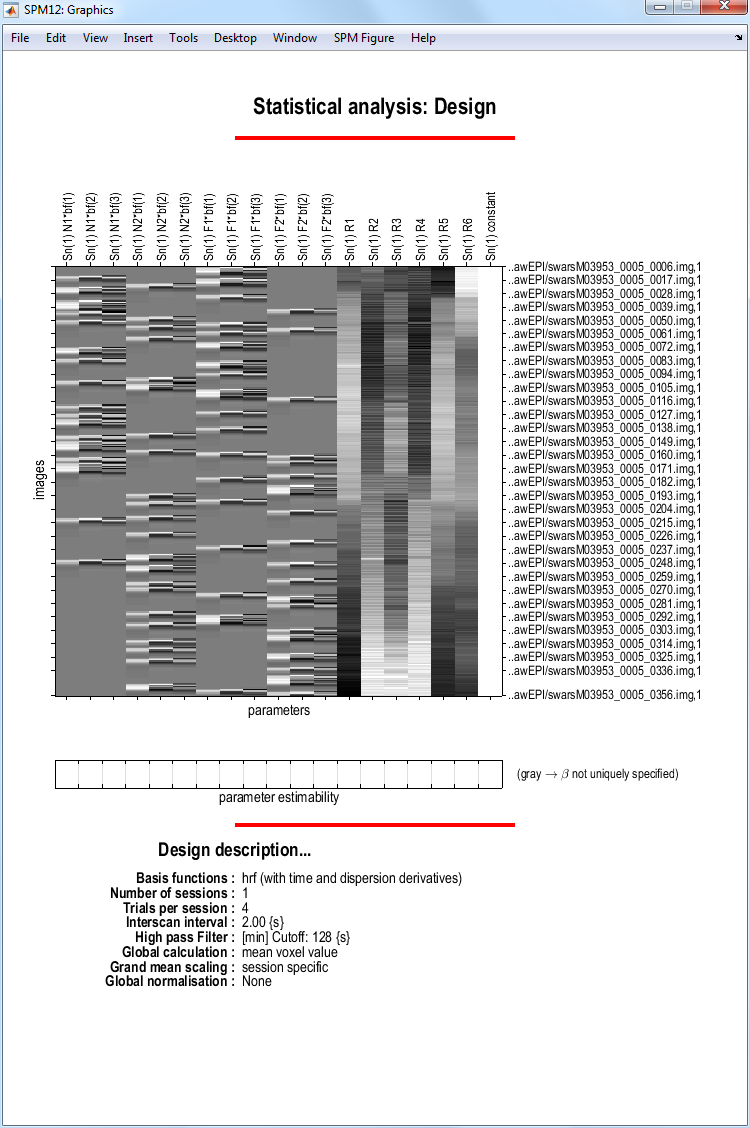
\includegraphics[width=100mm]{faces/cat_design}
\caption{\em Design matrix. \label{cat_design}}
\end{center}
\end{figure}

At this stage it is advisable to check your model specification
using SPM's review facility which is accessed via
the `Review' button. This brings up a `design' tab on the 
interactive window clicking on which produces a pulldown
menu. If you select the first item `Design Matrix' SPM will 
produce the image shown in Figure~\ref{cat_design}. 
If you select `Explore' then `Session 1' then `N1', SPM will produce 
the plots shown in Figure~\ref{cat_explore}.
\begin{figure}
\begin{center}
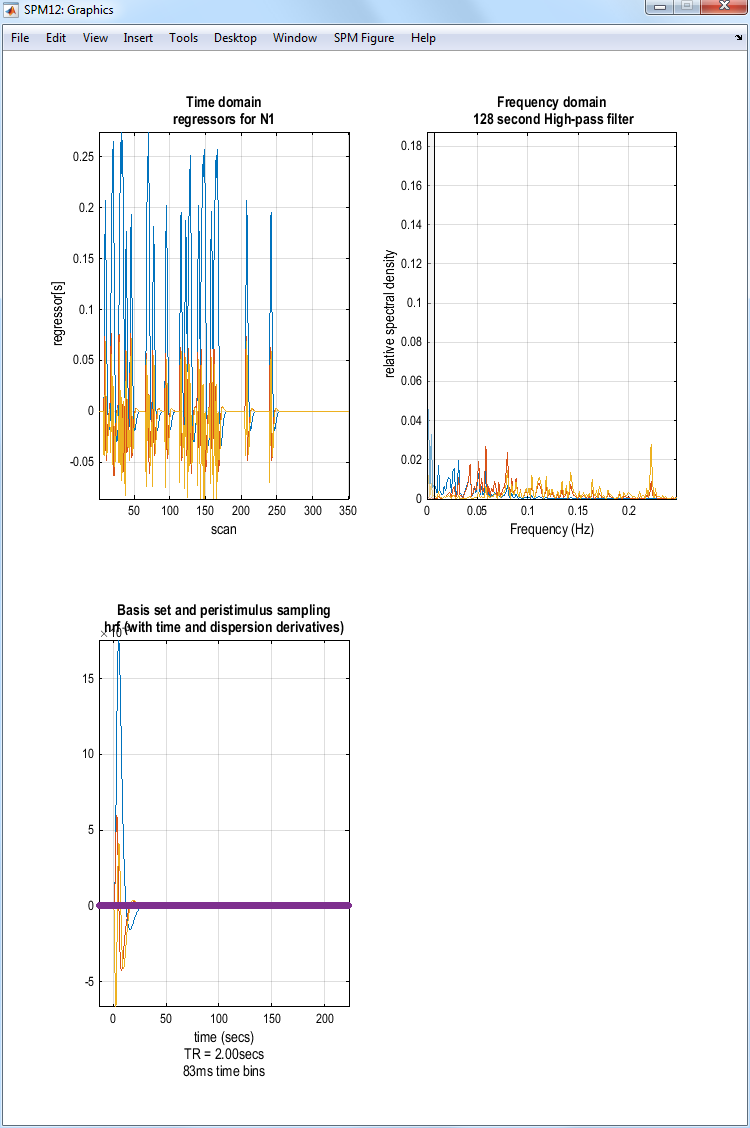
\includegraphics[width=100mm]{faces/cat_explore}
\caption{\em Exploring the design matrix in Figure~\ref{cat_design}. This shows the time series of 
the `active' regressor (top left), a frequency domain plot of the active regressor (top right) and 
the basis function used to convert assumed neuronal activity into hemodynamic activity. In this model 
we used the default option - the canonical basis function. The frequency domain plot shows that the 
frequency content of the `N1' regressor is above the set frequencies that are removed by the High Pass 
Filter (HPF) (these are shown in gray - in this model we accepted the default HPF cut-off of 128s or 
0.008Hz). \label{cat_explore}}
\end{center}
\end{figure}

\subsection{Estimate}

Press the `Estimate' button. This will call up the specification of an fMRI estimation job in the graphics window. Then
\bi
\item{Open the `fMRI model estimation' option}
\item{Highlight the `Select SPM.mat' option and then choose the SPM.mat
file saved in the \verb!DIR/categorical! directory}
\item{Save the job as \verb!categorical_est.job! and press Run}
\ei
SPM will write a number of files into the selected directory including 
an \verb!SPM.mat! file.

\subsection{Inference for categorical design}

Press `Results' and select the SPM.mat file from 
\verb!DIR\categorical!. This will again invoke the contrast manager. Because we specified that 
our model was using a `Factorial design' a number of 
contrasts have been specified automatically, as shown 
in Figure~\ref{cat_contrasts}.
\begin{figure}
\begin{center}
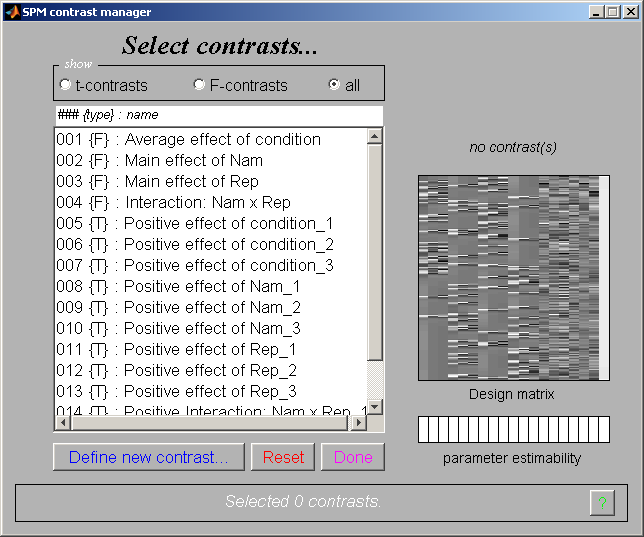
\includegraphics[width=100mm]{faces/cat_contrasts}
\caption{\em Contrast Manager containing default contrasts for categorical design. \label{cat_contrasts}}
\end{center}
\end{figure}

\bi
\item{Select contrast number 5. This is a t-contrast \verb!Positive effect of condition_1! This will show 
regions where the average effect of presenting faces is significantly positive, as modelled by 
the first regressor (hence the \verb!_1!), the 
canonical HRF. Press `Done'.}
\item{\em Mask with other contrast ? [Yes/No]}
\item{Specify No.}
\item{\em Title for comparison ?}
\item{Enter `Canonical HRF: Faces $>$ Baseline'}
\item{\em p value adjustment to control: [FWE/FDR/none]}
\item{Select FWE}
\item{\em Corrected p value(family-wise error)}
\item{Accept the default value, 0.05}
\item{\em Extent threshold \{voxels\} [0]}
\item{Accept the default value, 0}
\ei
SPM will then produce the MIP shown in Figure~\ref{cat5_volume}.

\subsection{Statistical tables}

To get a summary of local maxima, press the `Volume' button in the 
p-values section of the interactive window. This will list all clusters above the chosen level of significance as well as separate ($>$8mm apart) maxima within a cluster, with details of significance thresholds and search volume underneath, as shown in Figure~\ref{cat5_volume}
\begin{figure}
\begin{center}
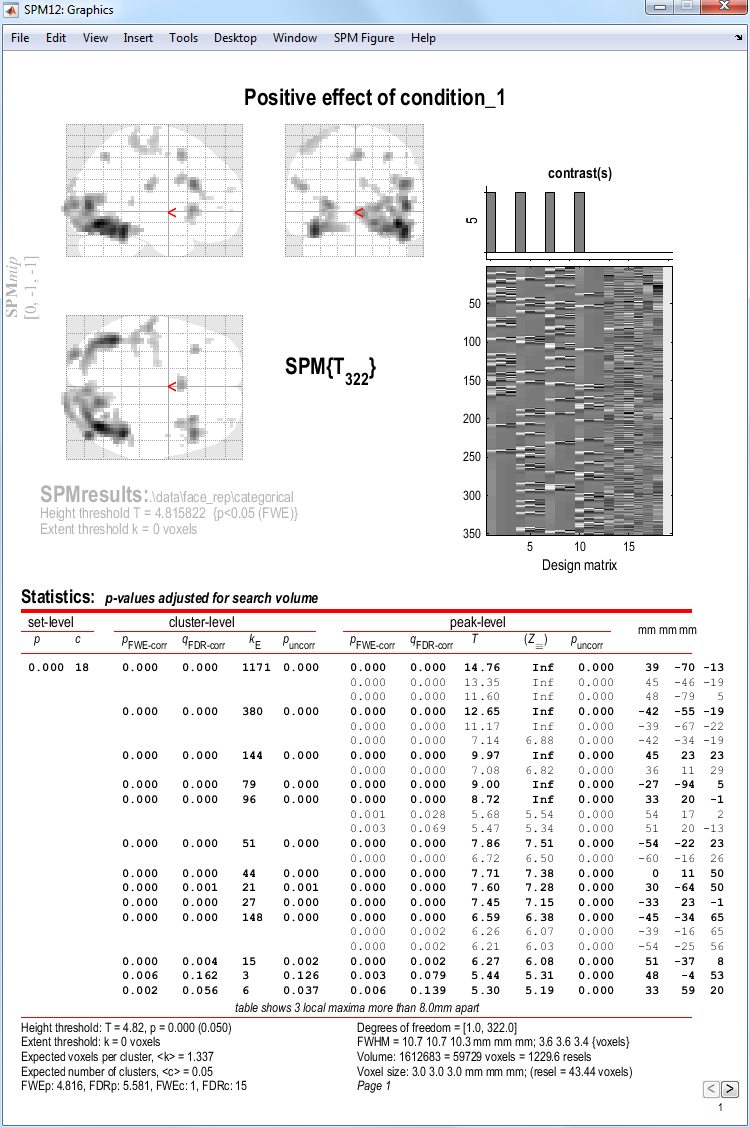
\includegraphics[width=100mm]{faces/cat5_volume}
\caption{\em MIP and Volume table for Canonical HRF: Faces  $>$ Baseline. \label{cat5_volume} }
\end{center}
\end{figure}
The columns in volume table show, from right to left:
\bi
\item{x, y, z (mm): coordinates in MNI space for each maximum}
\item{voxel-level: the chance (p) of finding (under the null hypothesis) a voxel with this or a greater height (T- or Z-statistic), corrected (FWE or FDR)/ uncorrected for search volume.}
\item{cluster-level: the chance (p) of finding a cluster with this many(ke) or a greater number of voxels, corrected / uncorrected for search volume}
\item{set-level: the chance (p) of finding this (c) or a greater number of clusters in the search volume}
\ei



\subsection{F-contrasts}

To assess the effect of presenting faces, as characterised by both the hrf {\em and} its temporal derivative, an F-contrast is required. Again, because we have told SPM that we have a factorial design, this required contrast will have been created automatically. 
\bi
\item{Press 'Results' and select the SPM.mat file in the 
\verb!DIR/categorical! directory}
\item{Select contrast number 1, as shown in Figure~\ref{cat1_contrast}. Press `Done'.}
\item{\em Mask with other contrast ? [Yes/No]}
\item{Specify No.}
\item{\em Title for comparison ?}
\item{Enter `HRF + deriv: Faces $>$ Baseline'}
\item{\em p value adjustment to control: [FWE/FDR/none]}
\item{Select FWE}
\item{\em Corrected p value(family-wise error)}
\item{Accept the default value, 0.05}
\item{\em Extent threshold \{voxels\} [0]}
\item{Accept the default value, 0}
\ei
Again, when the MIP appears, press 'Volume'. This should result in the display should in Figure~\ref{cat1_volume}.
\begin{figure}
\begin{center}
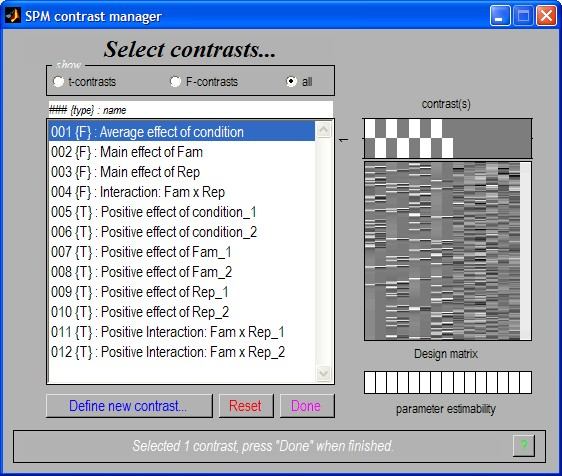
\includegraphics[width=100mm]{faces/cat1_contrast}
\caption{\em Contrast manager showing selection of the first contrast 'Average effect of condition', also known as `HRF + deriv: Faces  $>$ Baseline'. \label{cat1_contrast} }
\end{center}
\end{figure}

\begin{figure}
\begin{center}
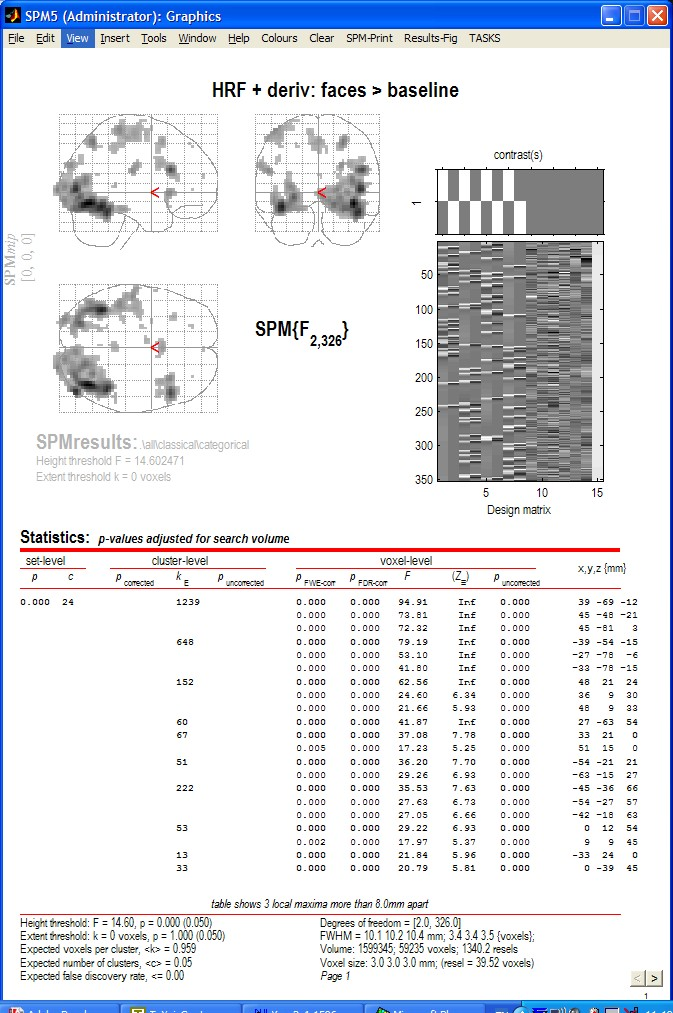
\includegraphics[width=100mm]{faces/cat1_volume}
\caption{\em MIP and Volume table for Canonical HRF: Faces  $>$ Baseline. \label{cat1_volume} }
\end{center}
\end{figure}
Although the MIP of this F-contrast looks similar to the previous t-contrast, note that the present contrast shows the areas for which the mean of the parameter estimates for the canonical hrf {\em or} its temporal derivative for the four conditions are different from zero (baseline). In other words, the F-contrast is two-sided, and tests two t-contrasts simultaneously. Also note that an F- (or t-) contrast such as [1 1 1 1 1 1 1 1], which tests whether the mean of the canonical hrf AND its temporal derivative for all conditions are different from (larger than) zero is not sensible. This is because the canonical hrf and its temporal derivative may cancel each other out while being significant in their own right. Finally, note that single F-contrasts can be regarded as $t^2$-contrasts, so that the F-contrasts [1 0 -1 0 1 0 -1 0] and [-1 0 1 0 -1 0 1 0] are equivalent. 

The relative contributions of the canonical hrf and its temporal derivative may also be assessed using the following F-contrast approach. This will allow us to plot the estimated effect sizes at a given voxel.
\bi
\item{Press `Results' and select the SPM.mat file in the 
\verb!DIR/categorical! directory}
\item{Press `Define new contrast', enter the name `All effects of interest', press the `F-contrast' radio button, enter [9:15] in the `columns in reduced design' window, press `OK', press `Done'.}
\item{\em Mask with other contrast ? [Yes/No]}
\item{Specify No.}
\item{\em Title for comparison ?}
\item{Accept what is offered}
\item{\em p value adjustment to control: [FWE/FDR/none]}
\item{Select FWE}
\item{\em Corrected p value(family-wise error)}
\item{Accept the default value, 0.05}
\item{\em Extent threshold \{voxels\} [0]}
\item{Accept the default value, 0}
\ei
Again, when the MIP appears, press 'Volume'. This should result in the display should in Figure~\ref{cat_all_volume}.
\begin{figure}
\begin{center}
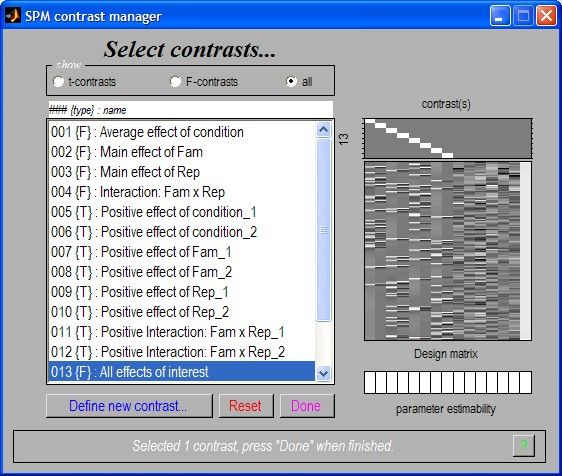
\includegraphics[width=100mm]{faces/cat_all_contrast}
\caption{\em Contrast manager showing specification of `All effects of interest'. \label{cat_all_contrast} }
\end{center}
\end{figure}

\begin{figure}
\begin{center}
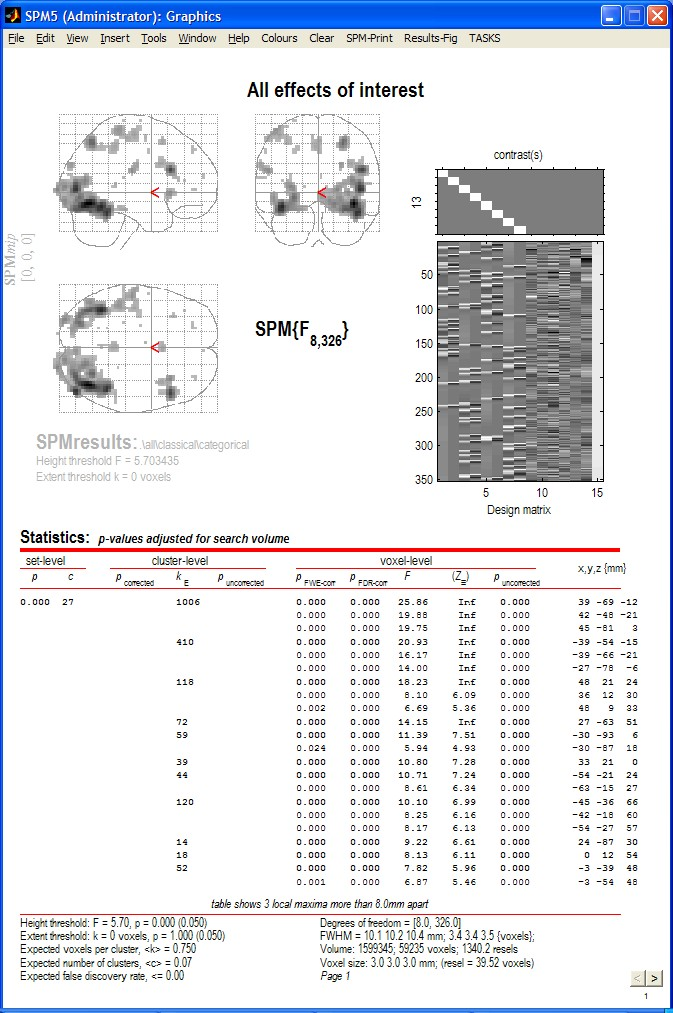
\includegraphics[width=100mm]{faces/cat_all_volume}
\caption{\em MIP and Volume table for `All effects of interest'. \label{cat_all_volume} }
\end{center}
\end{figure}


 

\subsection{Plotting parameter estimates at a voxel}

Move the cursor to e.g. the anterior right fusiform blob (the R fusiform face area) by clicking the second set of coordinates in the cluster (45 -48 -21) and press the `plot' button in SPM's interactive window. Select `Contrast of estimates and 90\% CI' and select 'All effects of interest'. This will produce the plot in 
Figure~\ref{con_all_plot}.
\begin{figure}
\begin{center}
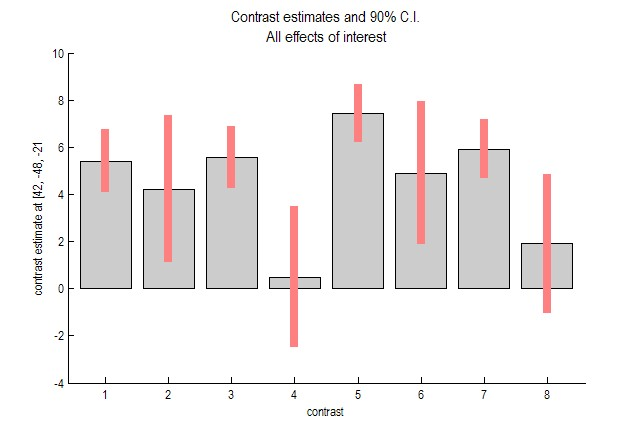
\includegraphics[width=100mm]{faces/con_all_plot}
\caption{\em Estimated effect sizes and 90\% confidence intervals for all effects of interest. Columns 1,3,5,7 are the canonical hrfs for N1 (non-famous faces, first presentation), N2 (non-famous faces, second presentation), F1 (famous faces, 1st presentation) and F2 (famous faces, 2nd presentation), whereas columns 2,4,6,8 are the temporal derivatives. \label{con_all_plot} }
\end{center}
\end{figure}
A positive coefficient for the canonical indicates a 
positive response to faces, whereas a positive coefficient for the derivative indicates a later peak 
response to faces. 
 Note, however, the large amplitudes and smaller error bars of the canonical hrfs compared to the temporal derivatives. This suggests that, for this region at least, the timing of the canonical model is adequate. Also note the repetition x stimulus type interaction; F1 seems larger than F2, whereas there is no 
 difference between N1 and N2. 


\subsection{F-contrasts for testing effects of movement}

To assess movement-related activation
\bi
\item{Press `Results', select the SPM.mat file, select 'F-contrast' in the Contrast Manager. Specify e.g. 'Rotation-related activation' (name) and 
in the 'contrasts weights matrix' window, or '1:11 15' in the 'columns for reduced design' window.} 
\item{
Submit and select the contrast, specify `mask with other contrasts?' (no), `title for comparison' (accept default), `corrected height threshold' (FWE), and `corrected p-value' (accept default).}
 \item{When the MIP appears, select `sections' from the `overlays' pulldown
 menu, and select the normalised structural image
 \verb!wmsM03953_0007.img!}
 \ei
\begin{figure}
\begin{center}
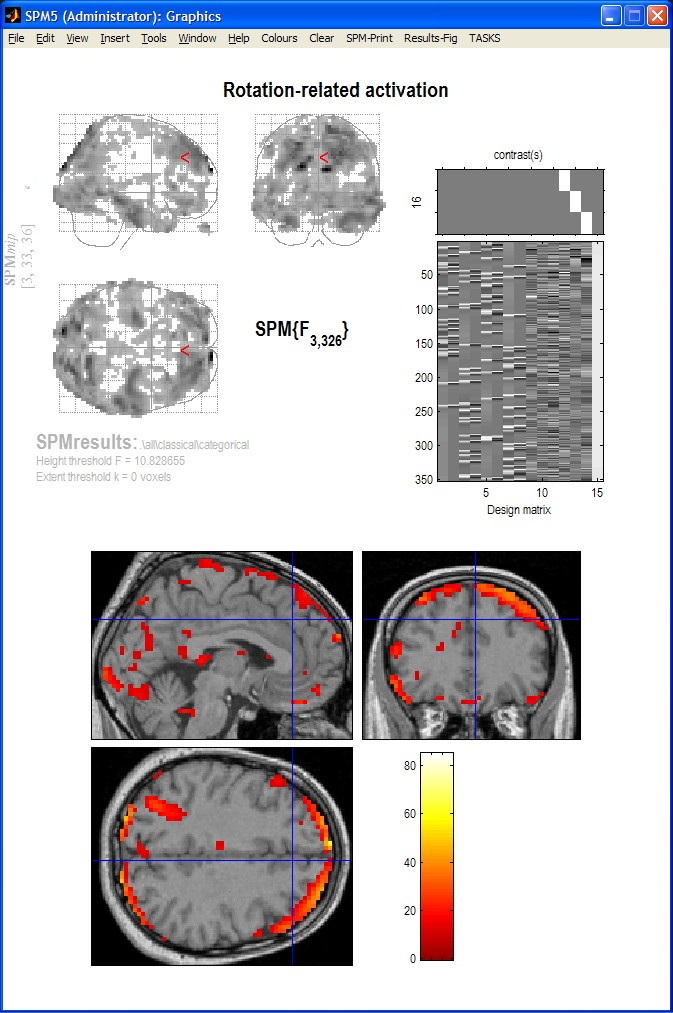
\includegraphics[width=100mm]{faces/rotations}
\caption{\em Rotation-related activations. These spurious `activations' are due to rotation of the head during scanning. These effects occur at tissue boundaries and boundaries between brain and non-brain, as this is where contrast differences 
are greatest. Including these regressors in the design matrix means these effects cannot be falsely attributed 
to neuronal activity. \label{rotations} }
\end{center}
\end{figure}

\section{Modelling parametric responses}

Before setting up the design matrix we must first 
load the Stimulus Onsets Times (SOTs), lag times, and movement
parameters into matlab. SOTs are stored in the 
\verb!sots.mat! file in a 
cell array such that eg. \verb!sot{1}! contains 
stimulus onset times in TRs for event type 1, which is N1. Event-types 2,3 and 4 are N2, F1 and F2\footnote{Also included included with this data set are variables describing two event-types of no interest - the (rare) errors made by this subject on the fame-judgement task. 
We will not, however, be using these in our analyses.}.

\bi
\item{At the matlab command prompt type \verb!load sots!. This loads the stimulus onset times (and the lag times).}
\ei

Now press the `Specify 1st-level' button. This will call up the specification of a fMRI specification job in the graphics window. Then
\bi
\item{Open the fMRI model specification option}
\item{Pres, `Load' and select the \verb!categorical_spec.mat! job file you created earlier}
\item{Open `Conditions' and then open the second `Condition'}
\item{Highlight `Parametric Modulations', select `New Parameter' and open the newly created `Parameter' option.}
\item{Highlight `Name' and enter 'Lag', highlight values and enter \verb!itemlag{2}!, highlight polynomial expansion and `2nd order'.}
\item{Now open the fourth `Condition' under `Conditions'}
\item{Highlight `Parametric Modulations', select `New Parameter' and open the newly created `Parameter' option.}
\item{Highlight `Name' and enter 'Lag', highlight values and enter \verb!itemlag{4}!, highlight polynomial expansion and `2nd order'.}
\item{Open `Canonical HRF' under `Basis Functions', highlight `Model derivatives' and select 
`No derivatives'.}
\item{Highlight `Directory' and select \verb!DIR/parametric!}
\item{Save the job as \verb!parametric_spec! and press `Run'}
\ei
This should produce the design matrix shown in Figure~\ref{par_design}.
\begin{figure}
\begin{center}
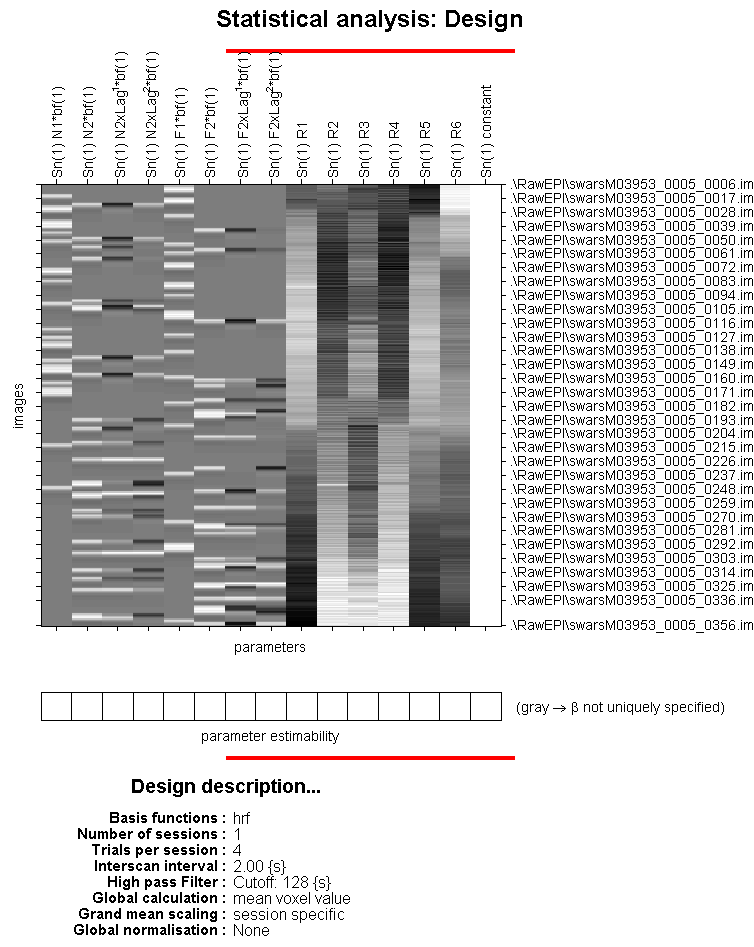
\includegraphics[width=100mm]{faces/par_design}
\caption{\em Design matrix for testing repetition effects parametrically. Regressor 2 indicates the second occurence of a nonfamous face. Regressor 3 modulates this linearly as a function of lag (ie. how many faces have been shown since that face was first presented), and regressor 4 modulates this quadratically as a function of lag. Regressors 6,7 and 8 play the same roles, but for famous faces. \label{par_design} }
\end{center}
\end{figure}

\subsection{Estimate}

Press the `Estimate' button. This will call up the specification of an fMRI estimation job in the graphics window. Then
\bi
\item{Open the `fMRI model estimation' option}
\item{Highlight the `Select SPM.mat' option and then choose the SPM.mat
file saved in the \verb!DIR/parametric! directory}
\item{Save the job as \verb!parametric_est.job! and press Run}
\ei
SPM will write a number of files into the selected directory including 
an \verb!SPM.mat! file.

\subsection{Plotting parametric responses}

To plot parametric responses, we first set up a contrast that captures positive responses to F2.
\bi
\item{Press `Results' and select the SPM.mat file in the 
\verb!DIR/parametric! directory}
\item{Press `Define new contrast', enter the name `Pos F2', press the `t-contrast' radio button, enter 
the contrast [0 0 0 0 0 1], press `submit', press `Done'.}
\item{\em Mask with other contrast ? [Yes/No]}
\item{Specify No.}
\item{\em Title for comparison ?}
\item{Accept what is offered}
\item{\em p value adjustment to control: [FWE/FDR/none]}
\item{Select FWE}
\item{\em Corrected p value(family-wise error)}
\item{Accept the default value, 0.05}
\item{\em Extent threshold \{voxels\} [0]}
\item{Accept the default value, 0}
\ei
We then set up a contrast that captures some 
parametric modulation of F2.
\bi
\item{Press `Results' and select the SPM.mat file in the 
\verb!DIR/parametric! directory}
\item{Press `Define new contrast', enter the name `Famous Lag', press the `F-contrast' radio button, enter `1:6 9:15' in the `columns in reduced design' window, press `submit', `OK' and `Done'.}
\item{\em Mask with other contrast ? [Yes/No]}
\item{Specify No.}
\item{\em Title for comparison ?}
\item{Accept what is offered}
\item{\em p value adjustment to control: [FWE/FDR/none]}
\item{Select None}
\item{\em Threshold \{F or p value\}}
\item{Accept the default value, 0.001}
\item{\em Extent threshold \{voxels\} [0]}
\item{Accept the default value, 0}
\ei
Now we will look at the modulation but masking it to restrict our attention to positive F2 effects. To do this
\bi
\item{Press `Results' and select the SPM.mat file in the 
\verb!DIR/parametric! directory}
\item{Select the `Famous Lag' contrast.}
\item{\em Mask with other contrast ? [Yes/No]}
\item{Specify Yes.}
\item{Select the `Pos F2' contrast}
\item{Accept the 0.05 uncorrected mask p-value}
\item{Nature of Mask ? inclusive}
\item{\em Title for comparison ?}
\item{Accept what is offered}
\item{\em p value adjustment to control: [FWE/FDR/none]}
\item{Select None}
\item{\em Threshold \{F or p value\}}
\item{Accept the default value, 0.001}
\item{\em Extent threshold \{voxels\} [0]}
\item{Accept the default value, 0}
\ei
Figure~\ref{famous_lag_mip} shows the MIP and an
overlay of this parametric effect using overlays, sections and selecting the \verb!wmsM03953_0007.img! image. 
\begin{figure}
\begin{center}
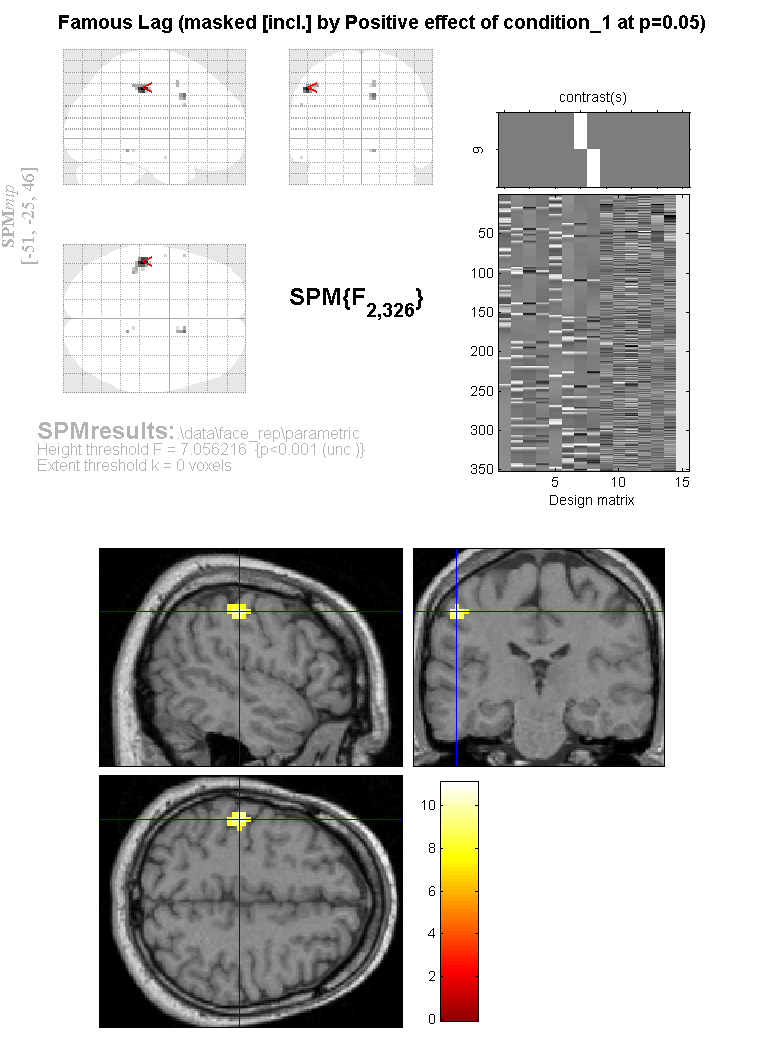
\includegraphics[width=100mm]{faces/famous_lag_mip}
\caption{\em MIP and overlay of parametric lag effect in parietal cortex. \label{famous_lag_mip} }
\end{center}
\end{figure}
The effect is plotted in the time domain in figure~\ref{famous_lag}. This was obtained by
\bi
\item{Right clicking on the MIP and selecting `global maxima'}
\item{Pressing Plot, and selecting `parametric responses' from the pull-down menu}
\item{Which effect ? select `F2'}
\ei
\begin{figure}
\begin{center}
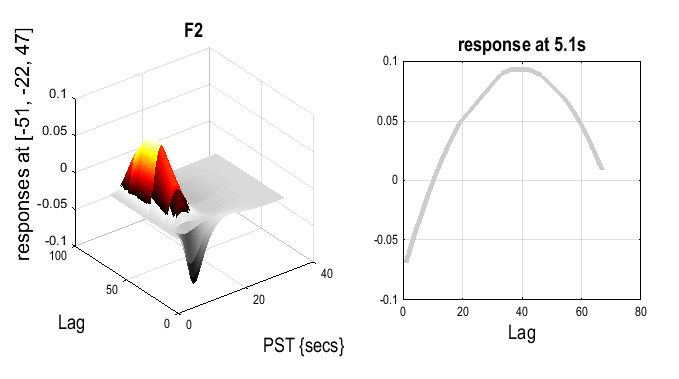
\includegraphics[width=150mm]{faces/famous_lag}
\caption{\em Response as a function of lag. \label{famous_lag} }
\end{center}
\end{figure}

\section{Bayesian analysis}

\subsection{Specification}

Press the `Specify 1st-level' button. This will call up an fMRI specification job in the graphics window. Then

\bi
\item{Open the fMRI model specification option}
\item{Load the \verb!categorical_spec.mat! job file created for the 
classical analysis}
\item{Open `Subject/Session', highlight `Scans'} \item{Deselect the smoothed functional images using the `unselect all' option available from a right mouse click in the SPM file selector (bottom window)}
\item{Select the 
unsmoothed functional images using the \verb!^w.*! filter and `select all' option available from a right mouse click in the SPM file selector (top right window)\footnote{Remember not to select the first 12 scans, scans 4 to 15, as these may contain T1 effects. This can be done during selection or by first moving the files to a different directory.}.
The Bayesian analysis uses a spatial prior where the spatial regularity in the signal is estimated from the data. It is therefore not necessary to create smoothed images if you are only going to do a Bayesian analysis.}
\item{Press `Done'}
\item{Highlight `Directory' and select the 
\verb!DIR/bayesian! directory you created earlier (you will first need to deselect the \verb!DIR/categorical! directory).}
\item{Save the job as \verb!specify_bayesian.mat! and press `Run'}
\ei

\subsection{Estimation}

Press the `Estimate' button. This will call up the specification of an fMRI estimation job in the graphics window. Then
\bi
\item{Open the `fMRI model estimation' option}
\item{Highlight the `Select SPM.mat' option and then choose the SPM.mat
file saved in the \verb!DIR\bayesian! subdirectory}
\item{Highlight `Method' and select the `Choose Bayesian 1st-level' option.}
\item{Save the job as \verb!estimate_bayesian.job! and press Run}
\ei
\begin{figure}
\begin{center}
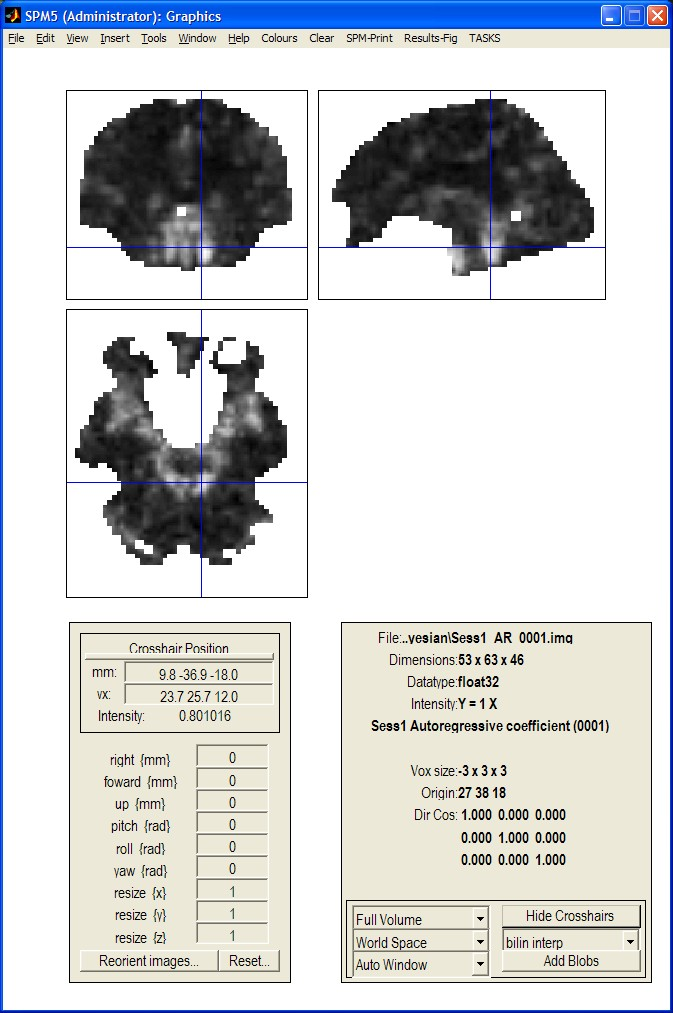
\includegraphics[width=100mm]{faces/face_ar1}
\caption{\em {\bf Bayesian analysis: Estimated AR(1) coefficient image indicating heterogeneity near the circle of Willis} \label{face_ar1} }
\end{center}
\end{figure}
SPM will write a number of files into the output directory including 
\bi
\item{An \verb!SPM.mat! file.}
\item{Images   \verb!Cbeta_000k.img! where $k$ indexes the $k$th estimated regression coefficient. These filenames are prefixed with a `C' indicating that these
are the mean values of the `Conditional' or `Posterior' density.}
\item{Images of error bars/standard deviations on the regression coefficients \verb!SDbeta_000k.img!.}
\item{An image of the standard deviation of the 
error \verb!Sess1_SDerror.img!.}
\item{An image \verb!mask.img! indicating which voxels 
were included in the analysis.}
\item{Images \verb!Sess1_AR_000p.img! where $p$ indexes the $p$th AR coefficient. See eg. Figure~\ref{face_ar1}.}
\item{Images \verb!con_000i.img! and \verb!con_sd_000i.img! which are the mean and standard deviation of the $i$th pre-defined contrast.} 
\ei

\subsection{Inference}

After estimation:

\bi
\item{Press `Results'}
\item{Select the \verb!SPM.mat! file created in the last section}
\item{Select contrast number 1: \verb!Positive effect of condition_1!, type `Done'.}
\item{\em Mask with other contrast ? [Yes/No]}
\item{Specify No}
\item{\em Title for comparison}
\item{Enter `Canonical HRF: Faces $>$ Baseline'}
\item{\em Effect size threshold for PPM}
\item{Enter the value 2}
\item{\em Posterior probability threshold for PPM}
\item{Enter the value 0.99}
\item{\em Extent threshold [0]}
\item{Accept the default value}
\item{\em Plot effect size [Yes/No]}
\item{Select the default `Yes'}
\ei
SPM will then plot a map of effect sizes at voxels 
where it is 99\% sure that the effect size is greater 
than 2\% of the global mean. This is a large activation.
Then use overlays, sections, select the 
normalised structural image created earlier and move the cursor to the activation in the left hemisphere. This should create the plot shown in Figure~\ref{face_bayes}

\begin{figure}
\begin{center}
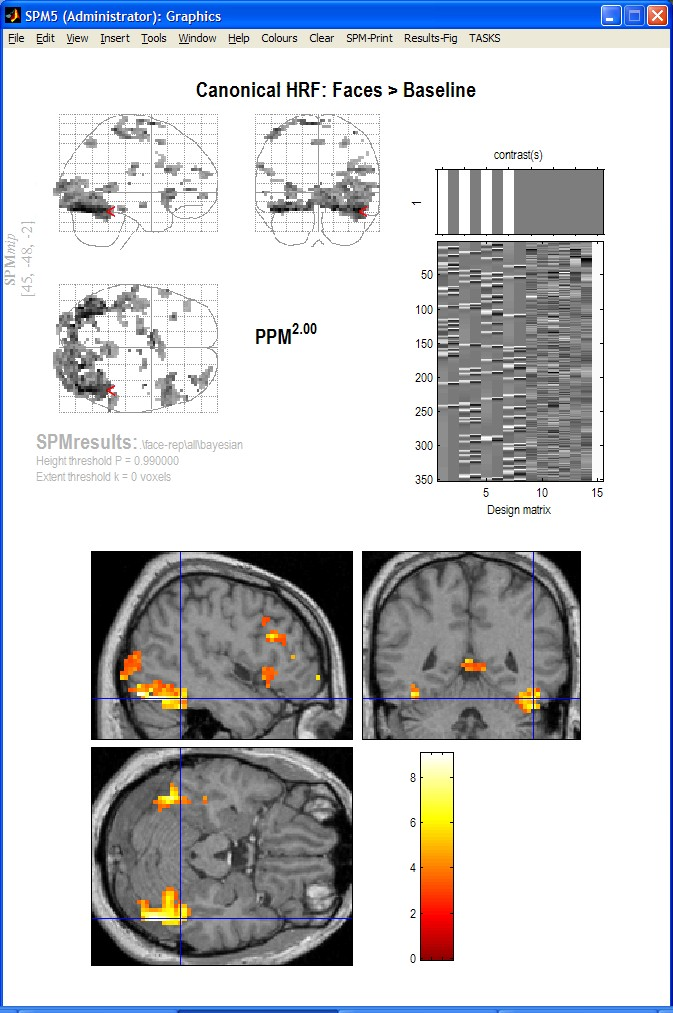
\includegraphics[width=100mm]{faces/face_bayes}
\caption{\em {\bf Bayesian analysis:} MIP and overlay of effect sizes at voxels 
where SPM is 99\% sure that the effect size is greater 
than 2\% of the global mean. The cursor is at the location $x=45,y=-48,z=-21$mm\label{face_bayes} }
\end{center}
\end{figure}


